% Created by tikzDevice version 0.12.6 on 2024-09-18 10:04:39
% !TEX encoding = UTF-8 Unicode
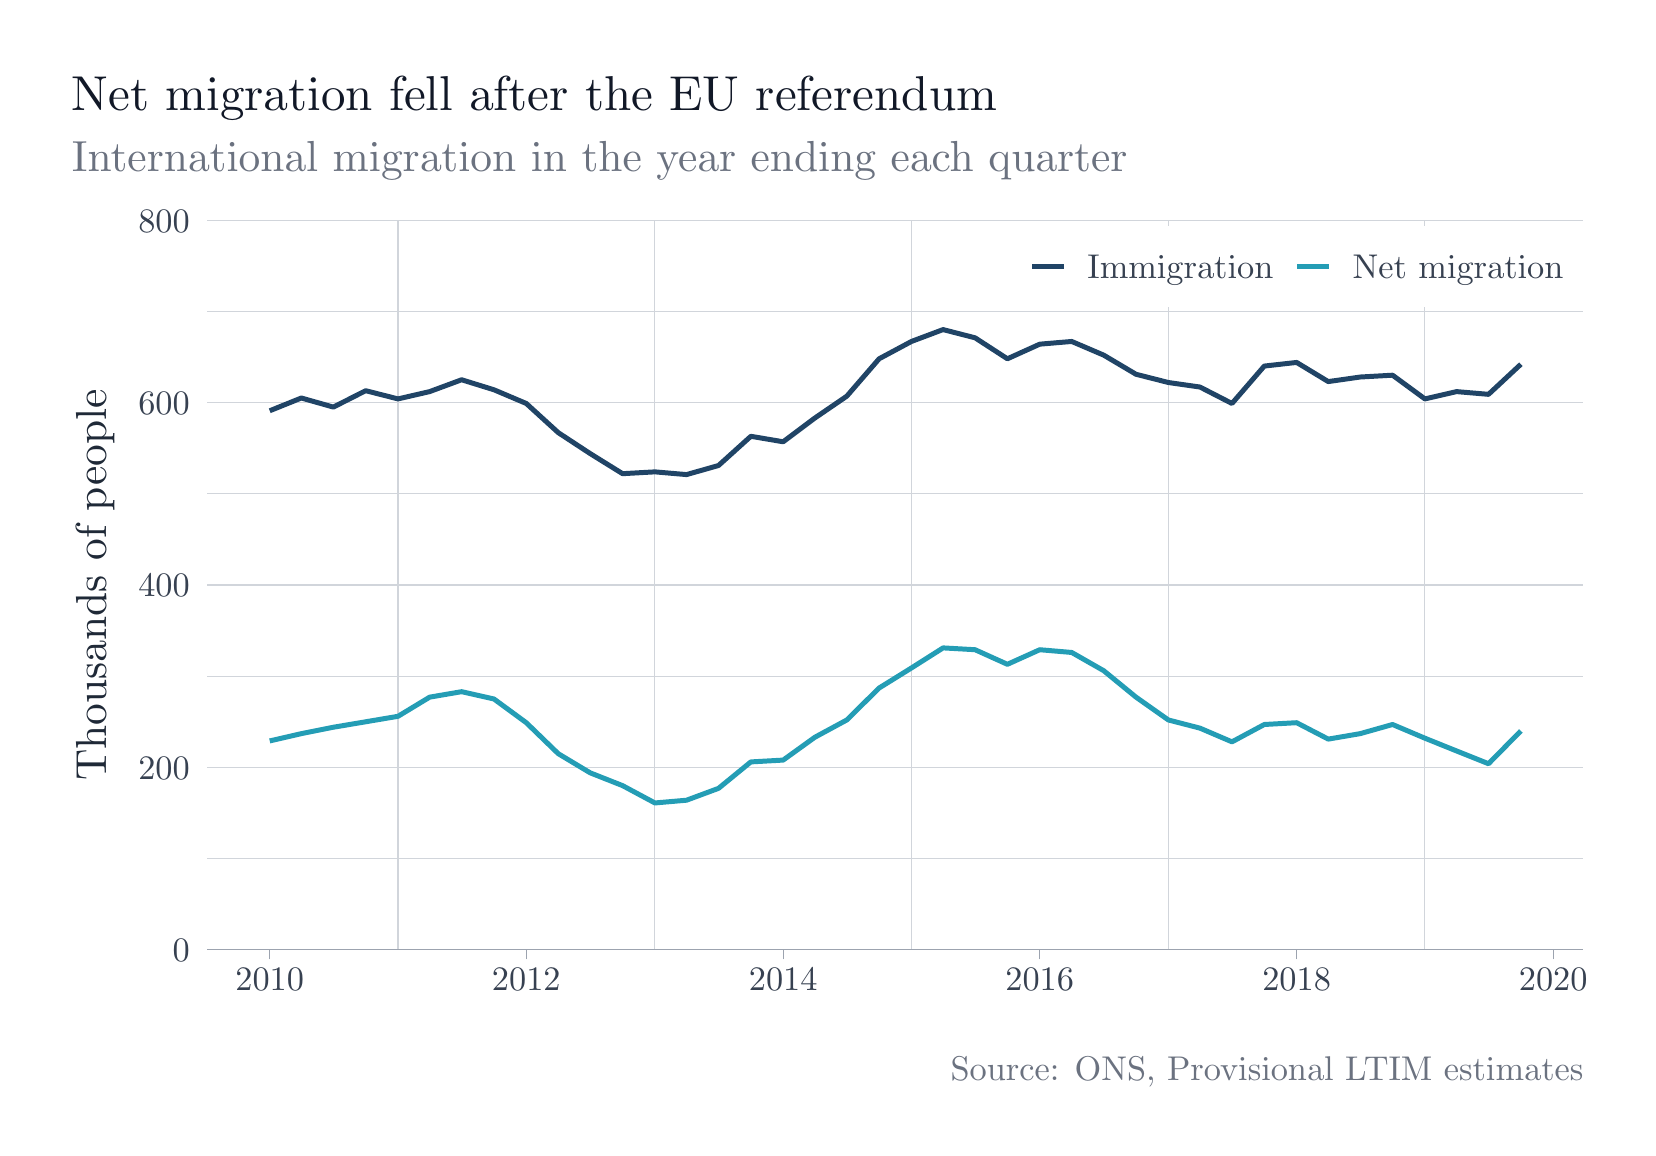
\begin{tikzpicture}[x=1pt,y=1pt]
\definecolor{fillColor}{RGB}{255,255,255}
\path[use as bounding box,fill=fillColor] (0,0) rectangle (578.16,397.48);
\begin{scope}
\path[clip] (  0.00,  0.00) rectangle (578.16,397.48);
\definecolor{drawColor}{RGB}{255,255,255}

\path[draw=drawColor,line width= 0.7pt,line join=round,line cap=round,fill=fillColor] (  0.00,  0.00) rectangle (578.16,397.48);
\end{scope}
\begin{scope}
\path[clip] ( 64.86, 64.27) rectangle (562.16,327.93);
\definecolor{drawColor}{RGB}{255,255,255}
\definecolor{fillColor}{RGB}{255,255,255}

\path[draw=drawColor,line width= 0.7pt,line join=round,line cap=round,fill=fillColor] ( 64.86, 64.27) rectangle (562.16,327.93);
\definecolor{drawColor}{RGB}{209,213,219}

\path[draw=drawColor,line width= 0.4pt,line join=round] ( 64.86, 97.23) --
	(562.16, 97.23);

\path[draw=drawColor,line width= 0.4pt,line join=round] ( 64.86,163.14) --
	(562.16,163.14);

\path[draw=drawColor,line width= 0.4pt,line join=round] ( 64.86,229.06) --
	(562.16,229.06);

\path[draw=drawColor,line width= 0.4pt,line join=round] ( 64.86,294.97) --
	(562.16,294.97);

\path[draw=drawColor,line width= 0.4pt,line join=round] (133.82, 64.27) --
	(133.82,327.93);

\path[draw=drawColor,line width= 0.4pt,line join=round] (226.59, 64.27) --
	(226.59,327.93);

\path[draw=drawColor,line width= 0.4pt,line join=round] (319.35, 64.27) --
	(319.35,327.93);

\path[draw=drawColor,line width= 0.4pt,line join=round] (412.12, 64.27) --
	(412.12,327.93);

\path[draw=drawColor,line width= 0.4pt,line join=round] (504.89, 64.27) --
	(504.89,327.93);

\path[draw=drawColor,line width= 0.4pt,line join=round] ( 64.86, 64.27) --
	(562.16, 64.27);

\path[draw=drawColor,line width= 0.4pt,line join=round] ( 64.86,130.19) --
	(562.16,130.19);

\path[draw=drawColor,line width= 0.4pt,line join=round] ( 64.86,196.10) --
	(562.16,196.10);

\path[draw=drawColor,line width= 0.4pt,line join=round] ( 64.86,262.01) --
	(562.16,262.01);

\path[draw=drawColor,line width= 0.4pt,line join=round] ( 64.86,327.93) --
	(562.16,327.93);
\definecolor{drawColor}{RGB}{32,68,102}

\path[draw=drawColor,line width= 1.8pt,line join=round] ( 87.47,259.05) --
	( 98.90,263.66) --
	(110.45,260.37) --
	(122.14,266.30) --
	(133.82,263.33) --
	(145.25,265.97) --
	(156.81,270.25) --
	(168.49,266.63) --
	(180.17,261.68) --
	(191.73,251.14) --
	(203.28,243.56) --
	(214.97,236.31) --
	(226.65,236.97) --
	(238.08,235.98) --
	(249.64,239.27) --
	(261.32,249.82) --
	(273.00,247.84) --
	(284.43,256.41) --
	(295.99,264.32) --
	(307.67,277.83) --
	(319.35,284.09) --
	(330.78,288.38) --
	(342.34,285.41) --
	(354.02,277.83) --
	(365.71,283.11) --
	(377.26,284.09) --
	(388.82,279.15) --
	(400.50,272.23) --
	(412.18,269.26) --
	(423.61,267.62) --
	(435.17,261.68) --
	(446.85,275.20) --
	(458.54,276.51) --
	(469.96,269.59) --
	(481.52,271.24) --
	(493.20,271.90) --
	(504.89,263.33) --
	(516.32,265.97) --
	(527.87,264.98) --
	(539.56,275.86);
\definecolor{drawColor}{RGB}{36,157,181}

\path[draw=drawColor,line width= 1.8pt,line join=round] ( 87.47,139.74) --
	( 98.90,142.38) --
	(110.45,144.69) --
	(122.14,146.66) --
	(133.82,148.64) --
	(145.25,155.56) --
	(156.81,157.54) --
	(168.49,154.90) --
	(180.17,146.33) --
	(191.73,135.13) --
	(203.28,128.21) --
	(214.97,123.59) --
	(226.65,117.33) --
	(238.08,118.32) --
	(249.64,122.61) --
	(261.32,132.16) --
	(273.00,132.82) --
	(284.43,141.06) --
	(295.99,147.32) --
	(307.67,158.86) --
	(319.35,166.11) --
	(330.78,173.36) --
	(342.34,172.70) --
	(354.02,167.43) --
	(365.71,172.70) --
	(377.26,171.71) --
	(388.82,165.12) --
	(400.50,155.56) --
	(412.18,147.32) --
	(423.61,144.36) --
	(435.17,139.41) --
	(446.85,145.68) --
	(458.54,146.33) --
	(469.96,140.40) --
	(481.52,142.38) --
	(493.20,145.68) --
	(504.89,140.73) --
	(516.32,136.12) --
	(527.87,131.50) --
	(539.56,143.37);
\end{scope}
\begin{scope}
\path[clip] (  0.00,  0.00) rectangle (578.16,397.48);
\definecolor{drawColor}{RGB}{55,65,81}

\node[text=drawColor,anchor=base east,inner sep=0pt, outer sep=0pt, scale=  1.24] at ( 58.56, 59.99) {0};

\node[text=drawColor,anchor=base east,inner sep=0pt, outer sep=0pt, scale=  1.24] at ( 58.56,125.90) {200};

\node[text=drawColor,anchor=base east,inner sep=0pt, outer sep=0pt, scale=  1.24] at ( 58.56,191.82) {400};

\node[text=drawColor,anchor=base east,inner sep=0pt, outer sep=0pt, scale=  1.24] at ( 58.56,257.73) {600};

\node[text=drawColor,anchor=base east,inner sep=0pt, outer sep=0pt, scale=  1.24] at ( 58.56,323.64) {800};
\end{scope}
\begin{scope}
\path[clip] (  0.00,  0.00) rectangle (578.16,397.48);
\definecolor{drawColor}{RGB}{156,163,175}

\path[draw=drawColor,line width= 0.3pt,line join=round] ( 64.86, 64.27) --
	(562.16, 64.27);
\end{scope}
\begin{scope}
\path[clip] (  0.00,  0.00) rectangle (578.16,397.48);
\definecolor{drawColor}{RGB}{156,163,175}

\path[draw=drawColor,line width= 0.3pt,line join=round] ( 87.47, 60.77) --
	( 87.47, 64.27);

\path[draw=drawColor,line width= 0.3pt,line join=round] (180.17, 60.77) --
	(180.17, 64.27);

\path[draw=drawColor,line width= 0.3pt,line join=round] (273.00, 60.77) --
	(273.00, 64.27);

\path[draw=drawColor,line width= 0.3pt,line join=round] (365.71, 60.77) --
	(365.71, 64.27);

\path[draw=drawColor,line width= 0.3pt,line join=round] (458.54, 60.77) --
	(458.54, 64.27);

\path[draw=drawColor,line width= 0.3pt,line join=round] (551.24, 60.77) --
	(551.24, 64.27);
\end{scope}
\begin{scope}
\path[clip] (  0.00,  0.00) rectangle (578.16,397.48);
\definecolor{drawColor}{RGB}{55,65,81}

\node[text=drawColor,anchor=base,inner sep=0pt, outer sep=0pt, scale=  1.24] at ( 87.47, 49.40) {2010};

\node[text=drawColor,anchor=base,inner sep=0pt, outer sep=0pt, scale=  1.24] at (180.17, 49.40) {2012};

\node[text=drawColor,anchor=base,inner sep=0pt, outer sep=0pt, scale=  1.24] at (273.00, 49.40) {2014};

\node[text=drawColor,anchor=base,inner sep=0pt, outer sep=0pt, scale=  1.24] at (365.71, 49.40) {2016};

\node[text=drawColor,anchor=base,inner sep=0pt, outer sep=0pt, scale=  1.24] at (458.54, 49.40) {2018};

\node[text=drawColor,anchor=base,inner sep=0pt, outer sep=0pt, scale=  1.24] at (551.24, 49.40) {2020};
\end{scope}
\begin{scope}
\path[clip] (  0.00,  0.00) rectangle (578.16,397.48);
\definecolor{drawColor}{RGB}{31,41,55}

\node[text=drawColor,rotate= 90.00,anchor=base,inner sep=0pt, outer sep=0pt, scale=  1.57] at ( 28.38,196.10) {Thousands of people};
\end{scope}
\begin{scope}
\path[clip] (  0.00,  0.00) rectangle (578.16,397.48);
\definecolor{drawColor}{RGB}{255,255,255}
\definecolor{fillColor}{RGB}{255,255,255}

\path[draw=drawColor,line width= 0.7pt,line join=round,line cap=round,fill=fillColor] (354.47,296.84) rectangle (562.16,325.29);
\end{scope}
\begin{scope}
\path[clip] (  0.00,  0.00) rectangle (578.16,397.48);
\definecolor{drawColor}{RGB}{255,255,255}
\definecolor{fillColor}{RGB}{255,255,255}

\path[draw=drawColor,line width= 0.7pt,line join=round,line cap=round,fill=fillColor] (361.47,303.84) rectangle (375.92,318.29);
\end{scope}
\begin{scope}
\path[clip] (  0.00,  0.00) rectangle (578.16,397.48);
\definecolor{drawColor}{RGB}{32,68,102}

\path[draw=drawColor,line width= 1.8pt,line join=round] (362.91,311.06) -- (374.48,311.06);
\end{scope}
\begin{scope}
\path[clip] (  0.00,  0.00) rectangle (578.16,397.48);
\definecolor{drawColor}{RGB}{255,255,255}
\definecolor{fillColor}{RGB}{255,255,255}

\path[draw=drawColor,line width= 0.7pt,line join=round,line cap=round,fill=fillColor] (457.32,303.84) rectangle (471.78,318.29);
\end{scope}
\begin{scope}
\path[clip] (  0.00,  0.00) rectangle (578.16,397.48);
\definecolor{drawColor}{RGB}{36,157,181}

\path[draw=drawColor,line width= 1.8pt,line join=round] (458.77,311.06) -- (470.33,311.06);
\end{scope}
\begin{scope}
\path[clip] (  0.00,  0.00) rectangle (578.16,397.48);
\definecolor{drawColor}{RGB}{55,65,81}

\node[text=drawColor,anchor=base west,inner sep=0pt, outer sep=0pt, scale=  1.24] at (382.92,306.78) {Immigration};
\end{scope}
\begin{scope}
\path[clip] (  0.00,  0.00) rectangle (578.16,397.48);
\definecolor{drawColor}{RGB}{55,65,81}

\node[text=drawColor,anchor=base west,inner sep=0pt, outer sep=0pt, scale=  1.24] at (478.78,306.78) {Net migration};
\end{scope}
\begin{scope}
\path[clip] (  0.00,  0.00) rectangle (578.16,397.48);
\definecolor{drawColor}{RGB}{107,114,128}

\node[text=drawColor,anchor=base west,inner sep=0pt, outer sep=0pt, scale=  1.57] at ( 16.00,345.46) {International migration in the year ending each quarter};
\end{scope}
\begin{scope}
\path[clip] (  0.00,  0.00) rectangle (578.16,397.48);
\definecolor{drawColor}{RGB}{17,24,39}

\node[text=drawColor,anchor=base west,inner sep=0pt, outer sep=0pt, scale=  1.77] at ( 16.00,367.56) {Net migration fell after the EU referendum};
\end{scope}
\begin{scope}
\path[clip] (  0.00,  0.00) rectangle (578.16,397.48);
\definecolor{drawColor}{RGB}{107,114,128}

\node[text=drawColor,anchor=base east,inner sep=0pt, outer sep=0pt, scale=  1.24] at (562.16, 17.21) {Source: ONS, Provisional LTIM estimates};
\end{scope}
\end{tikzpicture}
